\documentclass[a4paper,12pt]{article}
\usepackage[utf8]{inputenc}
\usepackage[margin=1in]{geometry}
\usepackage{titlesec}
\usepackage{array}
\usepackage{lmodern}
\usepackage{hyperref}
\usepackage{xcolor}
\usepackage{fancyhdr}
\usepackage{tikz}
\usepackage{multicol}
\usepackage{background}
\usepackage[T1]{fontenc}
%\usepackage[x11names]{xcolor}
%\usepackage[magyar]{babel}
\usepackage[textwidth=12cm,centering]{geometry}
\geometry{a4paper, margin=1in}

\newcommand*\wb[3]{%
  {\fontsize{#1}{#2}\usefont{T1}{custom}{xl}{n}#3}}
  
  %{\fontsize{#1}{#2}\usefont{U}{webo}{xl}{n}#3}}

% Hyperref színek beállítása
\hypersetup{
    colorlinks=true,
    linkcolor=blue,
    urlcolor=blue,
    pdftitle={Otthoni Rostgazdag Menü},
    pdfauthor={Budavári Mátyás},
    pdfcreator={LaTeX}
}

% Fejléc és lábléc beállítás
\pagestyle{fancy}
\fancyhf{}
\fancyhead[L]{\textbf{Otthoni Rostgazdag Menü}}
\fancyhead[R]{\today}
\fancyfoot[L]{budavariam}
\fancyfoot[R]{\thepage}

% Sordísz beállítása
\newcommand{\sordisz}{%
  \vspace{1em}
  \begin{center}
    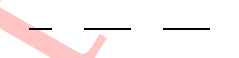
\begin{tikzpicture}
      \draw[thick] (0,0) -- (0.3,0);
      \draw[thick] (0.7,0) -- (1.3,0);
      \draw[thick] (1.7,0) -- (2.3,0);
    \end{tikzpicture}
  \end{center}
  \vspace{1em}
}

% The page frame
%\SetBgColor{Goldenrod3}
\SetBgColor{red}
\SetBgAngle{0}
\SetBgScale{1}
\SetBgOpacity{1}
\SetBgContents{%
\begin{tikzpicture}
\node at (0.5\paperwidth,0) {\wb{80}{34}{E}\rule[55pt]{.3\textwidth}{0.4pt}%
  \raisebox{50pt}{%
  \makebox[.4\textwidth]{\ \fontsize{24}{29}\selectfont\scshape Menü }}%
  \rule[55pt]{.3\textwidth}{0.4pt}\wb{80}{34}{F}};
\node at (2.4,-0.5\textheight) {\rule{0.4pt}{.82\textheight}};
\node at (19.1,-0.5\textheight) {\rule{0.4pt}{.82\textheight}};
\node at (0.5\paperwidth,-\textheight) {\wb{80}{80}{G}\rule[-10pt]{\textwidth}{0.4pt}\wb{80}{34}{H}} ;
\end{tikzpicture}%
}

% Dokumentum kezdete
\title{\Huge Otthoni Rostgazdag Menü}
\author{}
\date{}

\begin{document}

\maketitle
\tableofcontents
\newpage

\section{Hétfő és Kedd}
\sordisz
\subsection{Reggeli: Chia puding mandulatejjel}
\begin{itemize}
    \item 3 evőkanál chia mag
    \item 150 ml mandulatej
    \item Friss bogyós gyümölcsök (pl. áfonya, málna)
    \item 1 evőkanál mandula vagy dió
\end{itemize}
\textbf{Kalória:} 250 kcal \\
\textbf{Rost:} 10 g \\
\textbf{Elkészítés:} Áztasd be a chia magot mandulatejbe, hagyd állni 15-20 percig, majd keverd össze gyümölcsökkel és dióval.

\sordisz
\subsection{Ebéd: Sütőtökleves pirított tökmaggal}
\begin{itemize}
    \item 500 g sütőtök
    \item 1 fej vöröshagyma
    \item 2 gerezd fokhagyma
    \item 500 ml zöldségalaplé
    \item 2 evőkanál tökmag
    \item Teljes kiőrlésű kenyér
\end{itemize}
\textbf{Kalória:} 300 kcal \\
\textbf{Rost:} 8 g \\
\textbf{Elkészítés:} A sütőtököt és hagymát pirítsd meg, majd főzd meg alaplében, és turmixold össze. Szórd meg pirított tökmaggal.

\sordisz
\subsection{Vacsora: Lencsesaláta sült zöldségekkel}
\begin{itemize}
    \item 200 g főtt lencse
    \item 1 db répa
    \item 1 db cékla
    \item 1 db paprika
    \item 1 evőkanál dió
\end{itemize}
\textbf{Kalória:} 350 kcal \\
\textbf{Rost:} 12 g \\
\textbf{Elkészítés:} A zöldségeket süsd meg, majd keverd össze a lencsével és dióval.

\newpage

\section{Szerda és Csütörtök}
\sordisz
\subsection{Reggeli: Avokádós pirítós}
\begin{itemize}
    \item 1 szelet teljes kiőrlésű kenyér
    \item Fél avokádó
    \item Só, bors, citromlé
\end{itemize}
\textbf{Kalória:} 200 kcal \\
\textbf{Rost:} 7 g \\
\textbf{Elkészítés:} Az avokádót törd össze, keverd össze a fűszerekkel, majd kend a pirítósra.

\sordisz
\subsection{Ebéd: Quinoasaláta fekete babbal és kukoricával}
\begin{itemize}
    \item 150 g főtt quinoa
    \item 100 g fekete bab
    \item 50 g főtt kukorica
    \item Friss koriander, citromlé
\end{itemize}
\textbf{Kalória:} 400 kcal \\
\textbf{Rost:} 15 g \\
\textbf{Elkészítés:} A hozzávalókat keverd össze, és ízesítsd friss korianderrel és citromlével.

\sordisz
\subsection{Vacsora: Brokkoli krémleves}
\begin{itemize}
    \item 300 g brokkoli
    \item 1 db krumpli
    \item 500 ml zöldségalaplé
    \item 1 evőkanál olívaolaj
\end{itemize}
\textbf{Kalória:} 250 kcal \\
\textbf{Rost:} 9 g \\
\textbf{Elkészítés:} A brokkolit és a krumplit főzd meg alaplében, majd turmixold össze. Cseppents rá olívaolajat.

\newpage

\section{Péntek}
\sordisz
\subsection{Reggeli: Gyümölcssaláta dióval}
\begin{itemize}
    \item 1 db alma
    \item 1 db körte
    \item 1 marék szőlő
    \item 1 evőkanál dió
\end{itemize}
\textbf{Kalória:} 200 kcal \\
\textbf{Rost:} 6 g \\
\textbf{Elkészítés:} A gyümölcsöket vágd össze, és szórd meg dióval.

\sordisz
\subsection{Ebéd: Paradicsomos-csicseriborsós ragu}
\begin{itemize}
    \item 200 g főtt csicseriborsó
    \item 1 doboz paradicsompüré
    \item 1 fej vöröshagyma
    \item 1 evőkanál olívaolaj
\end{itemize}
\textbf{Kalória:} 350 kcal \\
\textbf{Rost:} 13 g \\
\textbf{Elkészítés:} A hagymát pirítsd meg, add hozzá a paradicsompürét és a csicseriborsót, majd főzd össze.

\sordisz
\subsection{Vacsora: Grillezett zöldségek hummusszal}
\begin{itemize}
    \item Cukkini, padlizsán, paprika
    \item 2 evőkanál hummusz
\end{itemize}
\textbf{Kalória:} 300 kcal \\
\textbf{Rost:} 10 g \\
\textbf{Elkészítés:} A zöldségeket grillezd meg, és tálald hummusszal.

\newpage

\section{Szombat}
\sordisz
\subsection{Reggeli: Főtt tojás friss zöldségekkel}
\begin{itemize}
    \item 2 db tojás
    \item Uborka, paprika, paradicsom
\end{itemize}
\textbf{Kalória:} 180 kcal \\
\textbf{Rost:} 4 g \\
\textbf{Elkészítés:} A tojásokat főzd keményre, és tálald friss zöldségekkel.

\sordisz
\subsection{Ebéd: Rostban gazdag zöldségpörkölt lencsével}
\begin{itemize}
    \item 200 g főtt lencse
    \item 1 db répa
    \item 1 db cukkini
    \item 1 db paprika
    \item 1 fej vöröshagyma
    \item 2 gerezd fokhagyma
    \item 1 evőkanál olívaolaj
    \item 400 g paradicsomkonzerv
    \item Só, bors, pirospaprika
\end{itemize}
\textbf{Kalória:} 350 kcal \\
\textbf{Rost:} 15 g \\
\textbf{Elkészítés:}  
\begin{enumerate}
    \item A hagymát és fokhagymát vágd apróra, majd pirítsd meg az olívaolajon.
    \item Add hozzá a felkockázott répát, cukkinít és paprikát, majd pirítsd őket pár percig.
    \item Öntsd hozzá a paradicsomot, sózd, borsozd, és szórd meg pirospaprikával.
    \item Főzd 20-30 percig, míg a zöldségek megpuhulnak.
    \item Keverd hozzá a főtt lencsét, és hagyd, hogy a pörkölt még 10 percig összeforrjon.
\end{enumerate}


\sordisz
\subsection{Vacsora: Céklás saláta kecskesajttal}
\begin{itemize}
    \item 1 db cékla
    \item 50 g kecskesajt
    \item Rukkola
    \item Dió
\end{itemize}
\textbf{Kalória:} 250 kcal \\
\textbf{Rost:} 6 g \\
\textbf{Elkészítés:} A céklát reszeld le, keverd össze a kecskesajttal és rukkolával, majd szórd meg dióval.

\newpage

\section{Vasárnap}
\sordisz
\subsection{Reggeli: Főtt tojás friss zöldségekkel}
\begin{itemize}
    \item 2 db tojás
    \item Uborka, paprika, paradicsom
\end{itemize}
\textbf{Kalória:} 180 kcal \\
\textbf{Rost:} 4 g \\
\textbf{Elkészítés:} A tojásokat főzd keményre, és tálald friss zöldségekkel.

\sordisz
\subsection{Ebéd: Sütőtökös rakottas}
\begin{itemize}
    \item 500 g sütőtök
    \item 200 g darált csirkehús
    \item 100 ml tejföl
    \item 1 evőkanál zsemlemorzsa
\end{itemize}
\textbf{Kalória:} 420 kcal \\
\textbf{Rost:} 8 g \\
\textbf{Elkészítés:} A sütőtököt szeleteld fel és párold meg. Rétegezd a darált hússal és tejföllel, szórd meg zsemlemorzsával, majd süsd 180°C-on 25 percig.

\sordisz
\subsection{Vacsora: Zöldborsós tészta spenóttal}
\begin{itemize}
    \item 150 g teljes kiőrlésű tészta
    \item 100 g friss spenót
    \item 100 g zöldborsó
    \item 1 gerezd fokhagyma
    \item 1 evőkanál olívaolaj
\end{itemize}
\textbf{Kalória:} 350 kcal \\
\textbf{Rost:} 10 g \\
\textbf{Elkészítés:} A tésztát főzd meg. Az olívaolajon pirítsd meg a fokhagymát, add hozzá a spenótot és a zöldborsót, majd forgasd össze a főtt tésztával.

\newpage

\section*{Hozzávalók összesítése}
\sordisz
\begin{multicols}{2}
\begin{itemize}
    \item Chia mag (250 g)
    \item Mandulatej (2-3 liter)
    \item Friss bogyós gyümölcsök
    \item Dió (200 g)
    \item Görög joghurt (1 kg)
    \item Teljes kiőrlésű kenyér
    \item Tojás (12 db)
    \item Avokádó (3-4 db)
    \item Sütőtök
    \item Barna rizs
    \item Brokkoli
    \item Fekete bab
    \item Quinoa
    \item Cékla
    \item Répa
    \item Paprika
\    \item Padlizsán
\    \item Cukkini
    \item Hummusz
    \item Kecskesajt
    \item Rukkola
\end{itemize}
\end{multicols}

\end{document}
